% You must put english here to handle hyphenation correctly
% Please keep this line to avoid using the parameter from the previous article in the proceedings
\selectlanguage{english} % possible values : french, english

%\settitle[Analysis of iDRAC]{Analysis of integrated Dell Remote Access Controller's interactions with an operating system: the quest to the main memory}
\settitle[Analysis of iDRAC]{iDRACKAR, integrated Dell Remote Access Controller's Kind Approach to the RAM}
%\settitle[Analysis of iDRAC]{iDRACKAR, integrated Dell Remote Access Controller's Kind Access to the RAM}

\setauthor[N.~Iooss]{Nicolas Iooss\\
  \email{nicolas.iooss@ssi.gouv.fr}}

\institute{ANSSI}

% To handle authors with multiple institutions, you can use the following code:
%
%   \setauthor[M.~MonNom, A.~MonAutreNom]{MonPrenom MonNom\inst{1} \and AutrePrenom AutreNom\inst{2}\\
%     \email{monprenom.monnom@mycorp.com\\autreprenom.autrenom@mycorp.com}}
%
%   \institute{OrganismePourMonNom \and OrganismePourAutreNom}
%
% For \institute, the numbering is automatic (and starts at 1)


\maketitle
\index{Iooss, N.}

\begin{abstract}
While Baseboard Management Controllers (BMC) grow in popularity as solutions to manage and monitor servers remotely, several critical vulnerabilities targeting them have recently been found.
On servers manufactured by HP, it has been published that the compromise of the BMC enables attackers to read and write the memory of the main operating system through Direct Memory Access (DMA) channels.
As these communication channels are not specific to HP, it can be expected that a vulnerability allowing attackers to execute arbitrary code on a BMC from another manufacturer provides a similar access.

In 2018, a remote code execution vulnerability targeting Dell's BMC (named iDRAC) was published.
The access provided by the exploitation of the vulnerability puts attackers in a similar position to being in the datacenter with physical access to the server: they can watch the screen, use a keyboard and a mouse, reboot the server, etc. However, they cannot read or write the RAM of the server.
More precisely, nobody has described how the iDRAC could perform DMA to the main RAM of a server.

On a Dell PowerEdge server, the iDRAC has a low-level access to many hardware components, for example in order to monitor the power and temperature of the CPU.
It does not usually perform DMA with the main memory, but this might be possible to achieve if the iDRAC has access to the relevant hardware interfaces.
This article digs into the interfaces used by iDRAC 8 in order to find out whether it can access the main memory.
It also focuses on components that are more likely to provide such an access, like the virtual USB devices, the CPLD connected to the iDRAC and the PCIe device that previous iDRAC revisions exposed.
In the end, none of these devices seem to provide an access to the memory of the main operating system.
Nevertheless the iDRAC interracts with a H8S microcontroller that appears to be closely related to the PCIe bus.
The analysis of this new microcontroller is still a work in progress.
\end{abstract}

\section{Introduction}

Several server manufacturers have been developing systems to monitor and manage servers out-of-band, through a dedicated network interface and operating system.
These systems, called \emph{Baseboard Management Controller} (BMC), run on their dedicated processors and measure the performance of server components (temperature, power consumption, fans, state of memory, etc.).

Dell has been developing a BMC named \emph{Dell Remote Access Controller} (DRAC) at least since 1999.
This product was first a pluggable device and later became an integrated chipset on the server motherboard (with iDRAC~6).
Nowadays, every generation of Dell PowerEdge servers comes with a new revision of the chipset: iDRAC 7 appeared with the 12th generation (in 2012), iDRAC 8 with the 13th one (in 2014) and iDRAC 9 with the 14th one (in 2017).
Since iDRAC 6, the architecture and the capabilities of the iDRAC have changed several times.
For example Dell introduced in 2016 a HTML5 remote console (replacing a Java applet) and implemented the Redfish API (a standardised REST API over HTTPS to perform several operations related to system management).
% https://ctrlaltdell.wordpress.com/2016/05/10/html5-console-on-your-idrac7-and-idrac8/
% The HTML Console is included in the 2.30.30.30 update. The update is available now and it’s free.
% redfish: https://www.dell.com/support/article/fr/fr/frbsdt1/sln310624/redfish?lang=en
% 13G (iDRAC 8/7) 2.40.40.40 (PDF: octobre 2016); 14G (iDRAC 9) 3.00.00.00
Moreover, one of the most important changes with the release of iDRAC 9 has been the transition from a Renesas SuperH CPU (named SH4) to an ARMv7 CPU.

Nowadays, the firmware of iDRAC is similar to a usual Linux system.
It is based on a GNU/Linux kernel, uses systemd as its init system and OpenSSL library for cryptographic operations.
Over the years, several vulnerabilities have been found and fixed in iDRAC.
For example, a critical one was discovered last year, CVE-2018-1207.
It allows anyone to get a root shell and to execute arbitrary code on an iDRAC.
Using such a vulnerability, someone can get access to the iDRAC administration console and perform actions such as controlling the virtual keyboard and mouse, watching the content of the screen, inserting a virtual CD-ROM from a file, rebooting the managed server, and using the network interface controller dedicated to the iDRAC to communicate with neighbor systems.
These actions are similar to the ones that can be performed by attackers who managed to sneak into the datacenter and have physical access to the server.
Nevertheless, attackers executing code on an iDRAC are not next to a server, they are inside it.
This leads to the following question: from a root shell on an iDRAC system, is it possible to read data in the main physical memory of the server, to compromise passwords or cryptographic keys?
Is it possible to modify it?
Can the main operating system prevent such unintended accesses, like configuring an IOMMU\footnote{The Input-Output Memory Management Unit is a component that restricts the access to the main memory from devices.} appropriately?

Even though the iDRAC of a Dell server has a low-level access to many hardware components, it does not usually access the data located in the main memory.
This article therefore describes the interfaces used by iDRAC in order to find out whether it can access the main memory.
After a short description of the legitimate and documented capabilities provided by iDRAC, it focuses on components which are more likely to provide this access.
More precisely, it studies the devices shared between the iDRAC and the main operating system, such as some USB devices and the screen.
As these devices do not provide an access to the PCIe bus from the iDRAC, it continues by describing components that are more specific, such as the CPLD\footnote{The Complex Programmable Logic Device is a programmable logic device that can be used to implement algorithms without manufacturing a custom chipset.} that is used and a mysterious PCIe endpoint called ``PBI device''.
This analysis ends with the discovery of a file used by iDRAC's bootloader to flash a component called ``PCIe bridge''.
This file contains what seems to be code using an uncommon instruction set, H8S, as well as the 16-bit identifiers of some PCIe switches and bridges seen from the main operating system.
The analysis of this code is still a work in progress and it is unclear whether the component running the H8S code could perform DMA requests to the main memory.

As all promising leads have failed for now, the iDRAC does not seem to be able to directly access the PCIe bus in order to read the main memory.
It is not known whether such an access could be possible in an indirect way, for example by modifying the firmware of the PCIe bridge which is flashed by iDRAC's bootloader.

The work which is presented in this article has been made possible thanks to the ANSSI, which provided the author with a Dell PowerEdge R730 server (13th Generation).
This server came with iDRAC 8 version 2.40.40.40 and some vulnerabilities.
There are major differences with iDRAC 9 (like the CPU architecture), so it is expected that many aspects of what is written in this article do not apply to iDRAC 9 and future versions.

\section{State of the art}

Implementations of Baseboard Management Controllers (BMC) have been available for more than twenty years: Dell's first Remote Access Controllers (DRAC) existed at least since 1999, HP launched the ProLiant BL20p with its iLO (integrated Lights-Out) in 2002, Intel implemented the Active Management Technology (AMT) on its Management Engine (ME) that can be found on chipsets launched in 2005, etc.

Since the birth of these systems, many vulnerabilities have been discovered.
The most recent ones include an authentication bypass on AMT (CVE-2017-5689) and on iLO (CVE-2017-12542), several post-authentication remote code execution vulnerabilities on iLO (CVE-2017-12542, CVE-2018-7078 and CVE-2018-7105) and on iDRAC (CVE-2018-1207) and a heap corruption on iDRAC (CVE-2018-1000116).

Several BMC implement a set of specifications named Intelligent Platform Management Interface (IPMI). These specifications and their implementations have been studied in length over the years.
In 2013, Anthony Bonkoski, Russ Bielawski and J. Alex Halderman described several implementations (HP's iLO, Dell's iDRAC, Oracle's iLOM, and Lenovo's IMM) and some vulnerabilities targeting them~\cite{idrackar:usenix2013ipmi}.
In 2015, Felix Emmert analyzed the features provided by iDRAC 7 and wrote a short description of the firmware~\cite{idrackar:emmert2015idrac}.
In 2017, Mark Ermolov and Maxim Goryachy from Positive Technology presented at Black Hat Europe their research on Intel's ME and AMT~\cite{idrackar:bheu2017hack}.
The same year, CERT-FR published some guidelines related to IPMI configuration~\cite{idrackar:certfr2017ipmi}.
In 2018, Fabien Périgaud, Alexandre Gazet and Joffrey Czarny presented their work on HP's iLO at several conferences (Recon Brussels~\cite{idrackar:recon2018ilo}, SSTIC~\cite{idrackar:sstic2018ilo} and ZeroNights~\cite{idrackar:zeronights2018ilo}).
During the summer of 2018, Matias Soler, Sebastian Soler and Nico Waisman from Immunity, Inc. presented at Black Hat USA other vulnerabilities targeting HP's iLO and Dell's iDRAC~\cite{idrackar:bhus2018bmc}.
Among these vulnerabilities was CVE-2018-1207, allowing a remote unauthenticated user to get their code run as \texttt{root} on iDRAC.

Many published vulnerabilities resulted in the possibility of executing arbitrary code on a BMC.
Once this was achieved, an attacker could, depending on the platform:

\begin{itemize}
  \item steal local credentials used by the BMC (unencrypted account passwords on iLO, password hashes on iDRAC, etc.);
  \item connect to the virtual keyboard-video-mouse interface to interact with the main operating system;
  \item use the virtual keyboard-video-mouse and virtual media interfaces to reboot the server and run an arbitrary operating system;
  \item use Direct Memory Access (DMA) controllers to read or modify the content of the main physical memory (RAM), on iLO;
  \item transmit network traffic to devices connected to the same network, using the Ethernet interfaces that the BMC can use;
  \item upgrade BMC's firmware and other key components of a server, eventually with backdoored firmware images;
  \item etc.
\end{itemize}

The authors usually described what actions they achieved to perform and the internals of the vulnerabilities they used.
This approach enabled readers to consider the criticality of a vulnerability, while keeping a fair amount of shade about what was really possible to achieve once arbitrary code would be executed on a BMC.

For example, accessing the main memory from the BMC has been shown to be feasible on iLO.
However, it has not been described from a compromised iDRAC.
Does it mean that such an access is not possible?
If it was possible, it would be provided by a hardware component accessible from the iDRAC.
This is why, compared to other works, this article gives a greater focus on the hardware components of a server and less on the services that are available from the network.

%This article studies the iDRAC system more in depth in order to search for an answer to this question.
%As it is much more difficult to prove that the access is impossible than the opposite, this article...


\section{Discovery of an iDRAC 8 system}

\subsection{Services using standard protocols}

When iDRAC 8 is configured on a server, it provides many services for users to manage the server.
These services are implemented using several standard protocols:
\begin{itemize}
  \item HTTPS, used by the web server, which provides:
    \begin{itemize}
      \item a remote view of the screen using HTML5 WebSockets;
      \item a JSON:API\footnote{JSON:API is the name of a specification of building an Application Programming Interface in JavaScript Object Notation, \url{https://jsonapi.org/}.} endpoint implementing Redfish 1.0 API;
    \end{itemize}
  \item SSH, used by the command line interface (SMASH CLP);
  \item IPMI over UDP and SNMP, used by their respective services;
  \item IPMI over SMBus, used for communications between the main operating system and the iDRAC.
\end{itemize}

The study of these interfaces helps getting a better understanding of the low-level capacity of the iDRAC.

As described in previous publications~\cite{idrackar:usenix2013ipmi}, these interfaces may require a user to authenticate themself before performing actions.
For example, the main page of the web server consists in a form that asks for a user name and a password (figure~\ref{fig:idrackar:login-page}).

\begin{figure}[p]
  \centering
  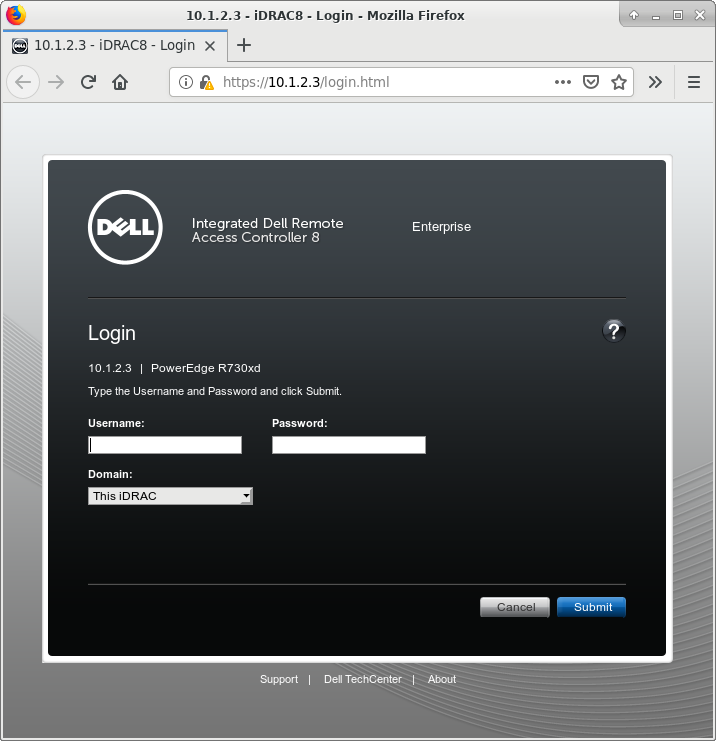
\includegraphics[width=0.6\textwidth]{03-idrackar/img/login-page.png}
  \caption{Login Page on iDRAC 8.}
  \label{fig:idrackar:login-page}
\end{figure}

\begin{figure}[p]
  \centering
  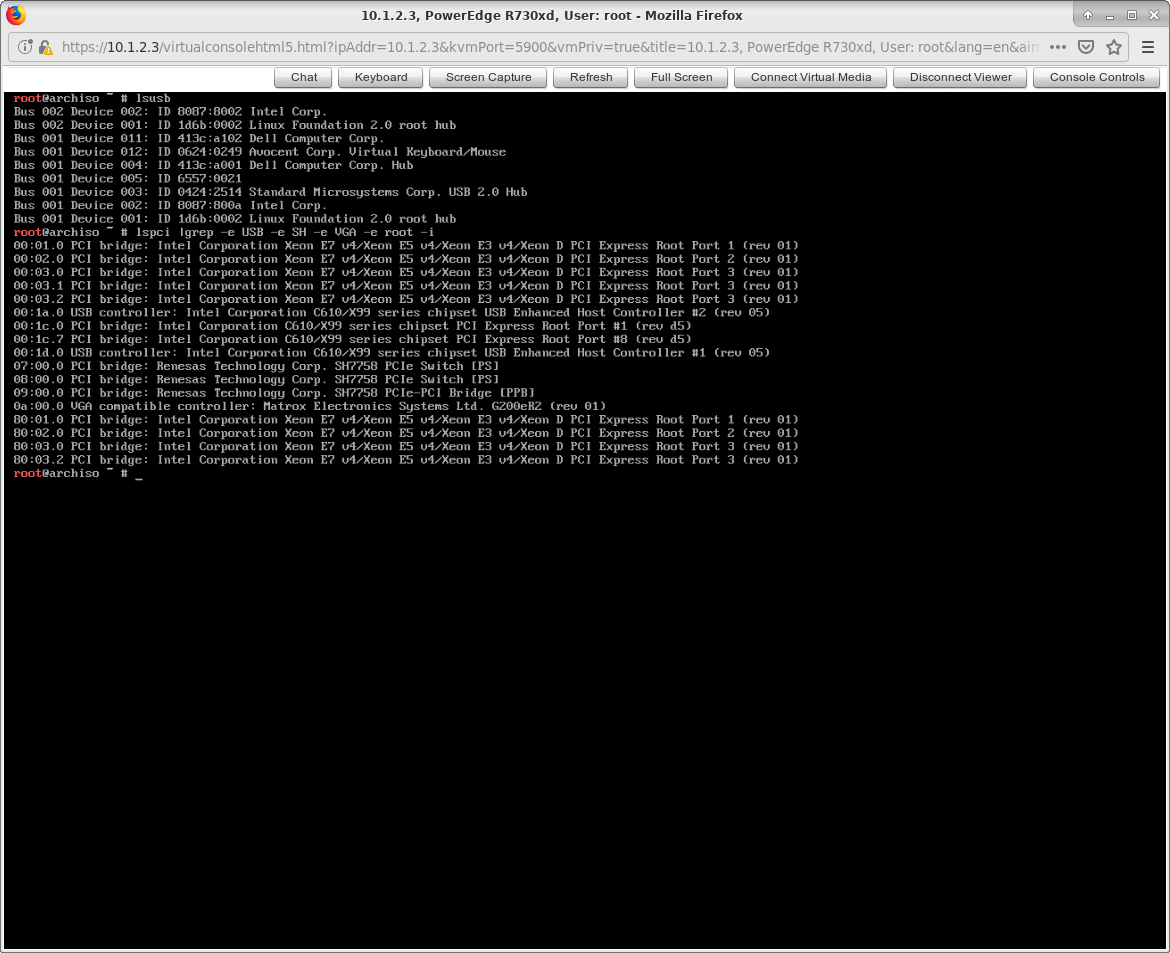
\includegraphics[width=0.9\textwidth]{03-idrackar/img/console-lspci-lsusb.png}
  \caption{Remote console on iDRAC 8.}
  \label{fig:idrackar:console-lspci-lsusb}
\end{figure}

Authenticated users can launch a virtual console (at URL \url{/virtualconsolehtml5.html}) in order to display the content of the screen of the server and to interact with it using their keyboards and mouses (figure~\ref{fig:idrackar:console-lspci-lsusb}).
The pressed keys and the mouse movements are transmitted through the web browser and the iDRAC to the main operating system, which sees them as coming from a USB-HID device named ``Avocent Keyboard/Mouse Function'' connected to a USB Hub named ``Dell Computer Corp. Hub''.
This means that the iDRAC is able to simulate some USB devices to the main operating system.
Section~\ref{sect:idrackar:hardware} gives more detail about this interaction.

From the authenticated part of the website, users can also reconfigure the iDRAC, trigger a reboot of the server, change the state of a UID LED\footnote{The \emph{Unit ID LED} is a light-emitting diode on a server that helps identifying it.}, etc.
All these features require the iDRAC to share access to some mainboard components with the main operating system.

The web server also implements Redfish 1.0 API under the URL \url{/redfish/v1/}.
This API enables an authenticated user to perform most of the actions provided by the BMC (monitor the server, add accounts to the iDRAC\footnote{Accounts can be added using the \url{/redfish/v1/Managers/iDRAC.Embedded.1/Accounts} endpoint.}, etc.) but in a way that is easier to integrate with programs.
On the web server used by iLO from HP, this interface has been vulnerable to an authentication bypass (CVE-2017-12542) and Périgaud, Gazet and Czarny published a way to fully compromise a HP server with it~\cite{idrackar:recon2018ilo}.
Even though this vulnerability did not exist on iDRAC, this proves the power of this API and the fact that iDRAC's web server needs a privileged access to the hardware components of a server.
The fact that Dell's implementation made the web server run as \texttt{root} can be related to this needed access.

The actions provided by Redfish API are also provided by the SMASH CLP (Systems Management Architecture for Server Hardware - Command Line Protocol) available over SSH.
Even though iDRAC uses a GNU/Linux kernel, the prompt that appears when a user authenticates to the iDRAC SSH server is a SMASH CLP prompt instead of a usual shell like \texttt{bash}.

\subsection{Firmware freedom}

Dell uses much free software in iDRAC.
This can be seen for example in the changelogs that are published with firmware updates.
For example, iDRAC 8's update to version 2.50.50.50\footnote{\url{https://www.dell.com/support/home/us/en/04/drivers/driversdetails?driverId=278FC}} contains changes such as ``Updated OpenSSH to 7.4p1'' and ``Upgraded to OpenSSL 1.0.2k''.
Moreover, Dell distributes the source code of these software, with the changes it did, in a place which can be found via the ``About'' page of iDRAC's website.
This page contains the following text:

\begin{quote}
  \footnotesize
  A portion of the software below may consist of open source software, which you can use as per the terms and conditions of the specific license under which the open source software is distributed.
  For certain open source software licenses, you are also entitled to obtain the corresponding source files.
  You may find corresponding source files for this program at \url{https://opensource.dell.com}.
\end{quote}

Several gigabytes of compressed data from iDRAC 8 components can indeed be downloaded from \url{https://opensource.dell.com/releases/idrac8/}.
Once extracted, this data contains:
\begin{itemize}
  \item the source code of some free-software projects used by iDRAC (in \texttt{externalsrc/}):
    \begin{itemize}
      \item the GNU/Linux kernel in \texttt{externalsrc/linux-yocto/}, with files specific to iDRAC's System-on-Chip (SoC), such as \texttt{arch/sh/boards/board-sh7757lcr.c}~;
      \item Dell's custom kernel modules used by iDRAC's firmware in \texttt{externalsrc/linux-drivers/}~;
      \item the U-Boot bootloader in \texttt{externalsrc/u-boot-idrac8/}, with files specific to iDRAC's SoC in the directory \texttt{u-boot\_B0/board/renesas/sh7757lcr/}~;
      \item OpenSSL, patches for OpenSSH, etc.;
    \end{itemize}
  \item many binary executable files (programs and shared libraries in ELF format), in \texttt{ipk-dropbox/}, that were compiled for a SH4 CPU;
  \item many other directories (\texttt{meta-drac}, \texttt{meta-oe}, \texttt{poky}, etc.).
\end{itemize}

The comments that are written in the distributed source code give a better understanding on how iDRAC firmware uses the hardware.

Furthermore, the firmware updates are not encrypted.
An update package for Linux consists in a shell script merged with an archive in tar.gz format.
This archive can be extracted using tools found in usual Linux systems (such as command \texttt{tar}).
It contains several tools that can be used on a Dell server running Linux to upgrade iDRAC's firmware using Linux's IPMI driver (through \texttt{/dev/ipmi0}).
The new firmware is located in file \texttt{payload/firmimg.d7} and contains a U-Boot image header, a Linux kernel, and two filesystems in Squashfs format that can be extracted using Binwalk.
One of the filesystems is the root filesystem of iDRAC, with usual directories (\texttt{/bin}, \texttt{/dev}, \texttt{/etc}, \texttt{/usr}, etc.).
Information about the Linux distribution that has been used in order to produce the firmware can be found in several files:
\begin{itemize}
  \item \texttt{/etc/issue} is ``\emph{Poky 8.0 (Yocto Project 1.3 Reference Distro) 1.3}'';
  \item \texttt{/bin/net-snmp-config} is a shell script containing options for \texttt{sh4-poky-linux-gcc}, such as \texttt{-{}-sysroot= /home/jenkins/jenkins\_slave\_builds\_prod/workspace/ idrac-13g-ducati1.5-master-release-A-Rev/ build-yocto-sh4/tmp/sysroots/idrac8};
  \item many binary files refer to this Jenkins directory when referencing paths to their source files.
\end{itemize}

As described on Poky's website\footnote{\url{https://www.yoctoproject.org/software-item/poky/}}, ``Poky is a reference distribution of the Yocto Project®''.
The Yocto Project® is a project whose goal is to produce tools and processes that enable the creation of Linux distributions for embedded and IoT software that are independent of the underlying architecture of the embedded hardware\footnote{\url{https://en.wikipedia.org/wiki/Yocto_Project}}.
The files that were found show that Poky is the distribution that Dell used in order to build iDRAC's firmware.

\subsection{Obtaining a shell}

Matias Soler, Sebastian Soler and Nico Waisman presented at Black Hat USA 2018 a way to exploit vulnerability CVE-2018-1207 in order to execute arbitrary commands on an iDRAC~\cite{idrackar:bhus2018bmc}.
This exploit enables attackers to upload a shared library through iDRAC's website and to load it in a process started from the browser.
Using functions that are executed as soon as the library is loaded, attackers can run arbitrary code as \texttt{root} on iDRAC.
The researchers used the exploit to launch a \emph{reverse-shell} from the web server (by establishing a TCP connection and binding it to a new instance of \texttt{/bin/sh}).
This shell is spawned as user \texttt{root}.
It would be easier to analyze the iDRAC if this shell was directly available via SSH.

The initial content of \texttt{/etc/passwd} is given on listing~\ref{lst:idrackar:original-passwd}.
The shell of \texttt{racuser} is \texttt{/usr/bin/clpd}, which is the program that implements the SMASH CLP.
Experiments show that \texttt{racuser} is the user that iDRAC uses to create processes resulting from a SSH connection\footnote{This behavior is caused by a patch allegedly written by Avocent and published by Dell in the releases available on \url{https://opensource.dell.com/releases/idrac8/} in file \texttt{meta-drac/recipes-yoctofixes/openssh/files/avocent.patch}.}.
After replacing \texttt{racuser}'s shell with \texttt{/bin/sh} (using the \emph{reverse-shell} obtained with CVE-2018-1207), when a user connects to the iDRAC through SSH, a real shell is launched instead of the SMASH CLP.

\begin{lstlisting}[language={},caption={original \texttt{/etc/passwd} from iDRAC firmware.},label={lst:idrackar:original-passwd}]
root:x:0:0:root:/:/bin/sh
user1:x:500:500:Linux User,,,:/:/bin/sh
racuser:x:1000:500:Linux User,,,:/tmp:/usr/bin/clpd
avahi:x:70:70:Avahi mDNS/DNS-SD Stack:/var/run/avahi-daemon:/sbin/nologin
sshd:x:74:74:Privilege-separated SSH:/var/empty/sshd:/bin/false
messagebus:x:999:997::/var/lib/dbus:/bin/false
_lldpd:x:1001:1001:Linux User,,,:/home/_lldpd:/bin/sh
\end{lstlisting}

Nevertheless, this shell runs as user \texttt{racuser}, which is not as privileged as \texttt{root}.
Thanks to command \texttt{su}, it is possible to spawn a privileged shell, but only if the password of the \texttt{root} account is known.
iDRAC's firmware update contains a file named \texttt{/etc/shadow} that holds the hashes of passwords (listing~\ref{lst:idrackar:original-shadow}).
The hash of \texttt{user1}'s password matches password ``\texttt{user1234}'', but \texttt{root}'s password does not seem to be publicly available, even though its hash was published a few years ago by Emmert~\cite{idrackar:emmert2015idrac}.

\begin{lstlisting}[language={},caption={original \texttt{/etc/shadow} from iDRAC firmware.},label={lst:idrackar:original-shadow}]
root:$1$fY6DG6Hu$OpwCBE01ILIS1H/Lxq/7d0:13502:0:99999:7:::
user1:$1$nVOr80rB$HDAd6FRlG24k/WN4ZuYPC0:0:0:99999:7:::
racuser:!:0:0:99999:7:::
avahi:!!:15569::::::
sshd:*:11880:0:99999:7:-1:-1:0
messagebus:!:15873:0:99999:7:::
_lldpd:!:16555:0:99999:7:::
\end{lstlisting}

Even though this password is unknown, the previous vulnerability allows overwriting its value in \texttt{/etc/shadow}.
This allows running a shell as \texttt{root} over SSH on the iDRAC.
Some commands can then be issued in order to collect precise information about the firmware version and iDRAC's environment, as shown in listing~\ref{lst:idrackar:root-shell}.

\begin{lstlisting}[language={},caption={some commands from a root shell on iDRAC 8.},label={lst:idrackar:root-shell}]
[SH7757 /flash/data0/home/root]$ su
root's password:

[SH7757 /flash/data0/home/root]$ id
uid=0(root) gid=0(root) groups=0(root)

[SH7757 /flash/data0/home/root]$ uname -a
Linux MpCOZlZ 3.4.11 #1 Thu Aug 18 13:03:21 CDT 2016 sh4a GNU/Linux

[SH7757 /flash/data0/home/root]$ cat /proc/version 
Linux version 3.4.11 (jenkins@gitbuild12g105) (gcc version 4.7.2 (GCC) ) #1 Thu Aug 18 13:03:21 CDT 2016

[SH7757 /flash/data0/home/root]$ cat /etc/issue
Poky 8.0 (Yocto Project 1.3 Reference Distro) 1.3 \n \l

[SH7757 /flash/data0/home/root]$ cat /flash/pd0/fw_ver
2.40.45.40.40
2.40.40.40.107
built for - system
Thu Aug 18 13:26:24 CDT 2016
160818132624
IDRAC SVN Rev  = 
Hudson Project = idrac-13g-ducati1.5-master-release-A-Rev
Hudson Build # = 619
Release ID     = 
MSC Revision = https://pgre-svn2.us.dell.com/svn/LC/13g/branches/rts_PlusPlusPlus/msc 4876

[SH7757 /flash/data0/home/root]$ cat /flash/pd0/lc_ver ; echo
2.40.40.40.107

[SH7757 /flash/data0/home/root]$ cat /proc/cpuinfo
machine         : SH7757LCR
processor       : 0
cpu family      : sh4a
cpu type        : SH7758
cut             : 11.x
cpu flags       : fpu perfctr llsc
cache type      : split (harvard)
icache size     : 32KiB (4-way)
dcache size     : 32KiB (4-way)
address sizes   : 32 bits physical
bogomips        : 576.00

[SH7757 /flash/data0/home/root]$ cat /proc/cmdline
root=/dev/mmcblk0p2 rootwait rw rootfstype=squashfs mem=239616k
console=ttyS2,115200 <NULL>
mac1=18:66:DA:XX:XX:XX mac2=18:66:da:xx:xx:xx
mode=normal reset_cause=ac nmi_buf=0x83000000 quiet
console=ttySC2,115200 init=/sbin/init

[SH7757 /flash/data0/home/root]$ ls -l /sbin/init
lrwxrwxrwx 1 root 0 20 Aug 18 2016 /sbin/init -> /lib/systemd/systemd
\end{lstlisting}

When exploring the system which is now accessible, something seems wrong: even though the iDRAC uses accounts (for its web interface, SMASH CLP, etc.), their usernames and passwords are different from the Linux user accounts.
This difference is caused by a custom configuration of PAM subsystem\footnote{The Pluggable Authentication Modules subsystem is a set of libraries and configuration files commonly used on Linux-based systems to authenticate users and manage sessions.}.
Indeed, \texttt{/etc/pam.d/} contains files that refer to modules \texttt{pam\_ldap\_manager.so} and \texttt{pam\_local\_manager.so} (listing~\ref{lst:idrackar:etc-pam-login}).

\begin{lstlisting}[language={},caption={extract from \texttt{/etc/pam.d/login} in iDRAC 8.},label={lst:idrackar:etc-pam-login}]
auth    sufficient  pam_ldap_manager.so
auth    sufficient  pam_local_manager.so use_first_pass
auth    required    pam_auth_status.so caller=login sessiontype=CLP
\end{lstlisting}

Library \texttt{/lib/security/pam\_local\_manager.so} uses functions from other libraries (\texttt{libosi.so.1.2.3}, \texttt{libaim.so.1.2.3} and \texttt{libfnmgr-client.so.9.9.9}) to verify account credentials, none of them related to the usual functions \texttt{getpwnam()} and \texttt{getspnam()} from glibc.
In the end, the account credentials are stored in a \emph{credential vault filesystem} which is configured by \texttt{/etc/init.d/credential-vault-13g.sh}.
This script mounts an encrypted file\footnote{The file is \texttt{/mmc1/.cv.img} and is mounted with \texttt{losetup}, \texttt{dmsetup create} and \texttt{mount}. The encryption cipher which is used is \texttt{aes-ecb-essiv:sha256} with a key that is hard-coded in script \texttt{/etc/init.d/credential-vault-13g.sh} and that does not seem to be customized in each installation.} on both \texttt{/flash/13g-cv} and \texttt{/flash/data0/cv}.
The credentials of iDRAC's accounts are located in \texttt{/flash/13g-cv/avctpasswd} and the passwords are hashed with salted SHA256\footnote{When considering each line of \texttt{/flash/13g-cv/avctpasswd} as a list of fields separated with ``\texttt{:}'', field \#0 is the username, field \#15 is a 16-byte-long salt encoded in hexadecimal and field \#14 is \texttt{SHA256(password || salt)} in hexadecimal.}.

\section{Hardware from a Linux point-of-view}
\label{sect:idrackar:hardware}

The previous section described the main services exposed by iDRAC, explained how the firmware and some source code can be downloaded and extracted, and presented a way to get a \texttt{root} shell on an iDRAC.
All of this enable studying iDRAC's interactions with the hardware of a server in order to find communication channels with the main operating system.

\subsection{The hardware seen from the main operating system}
\label{sect:idrackar:hardware-from-os}

\begin{figure}[p]
  \centering
  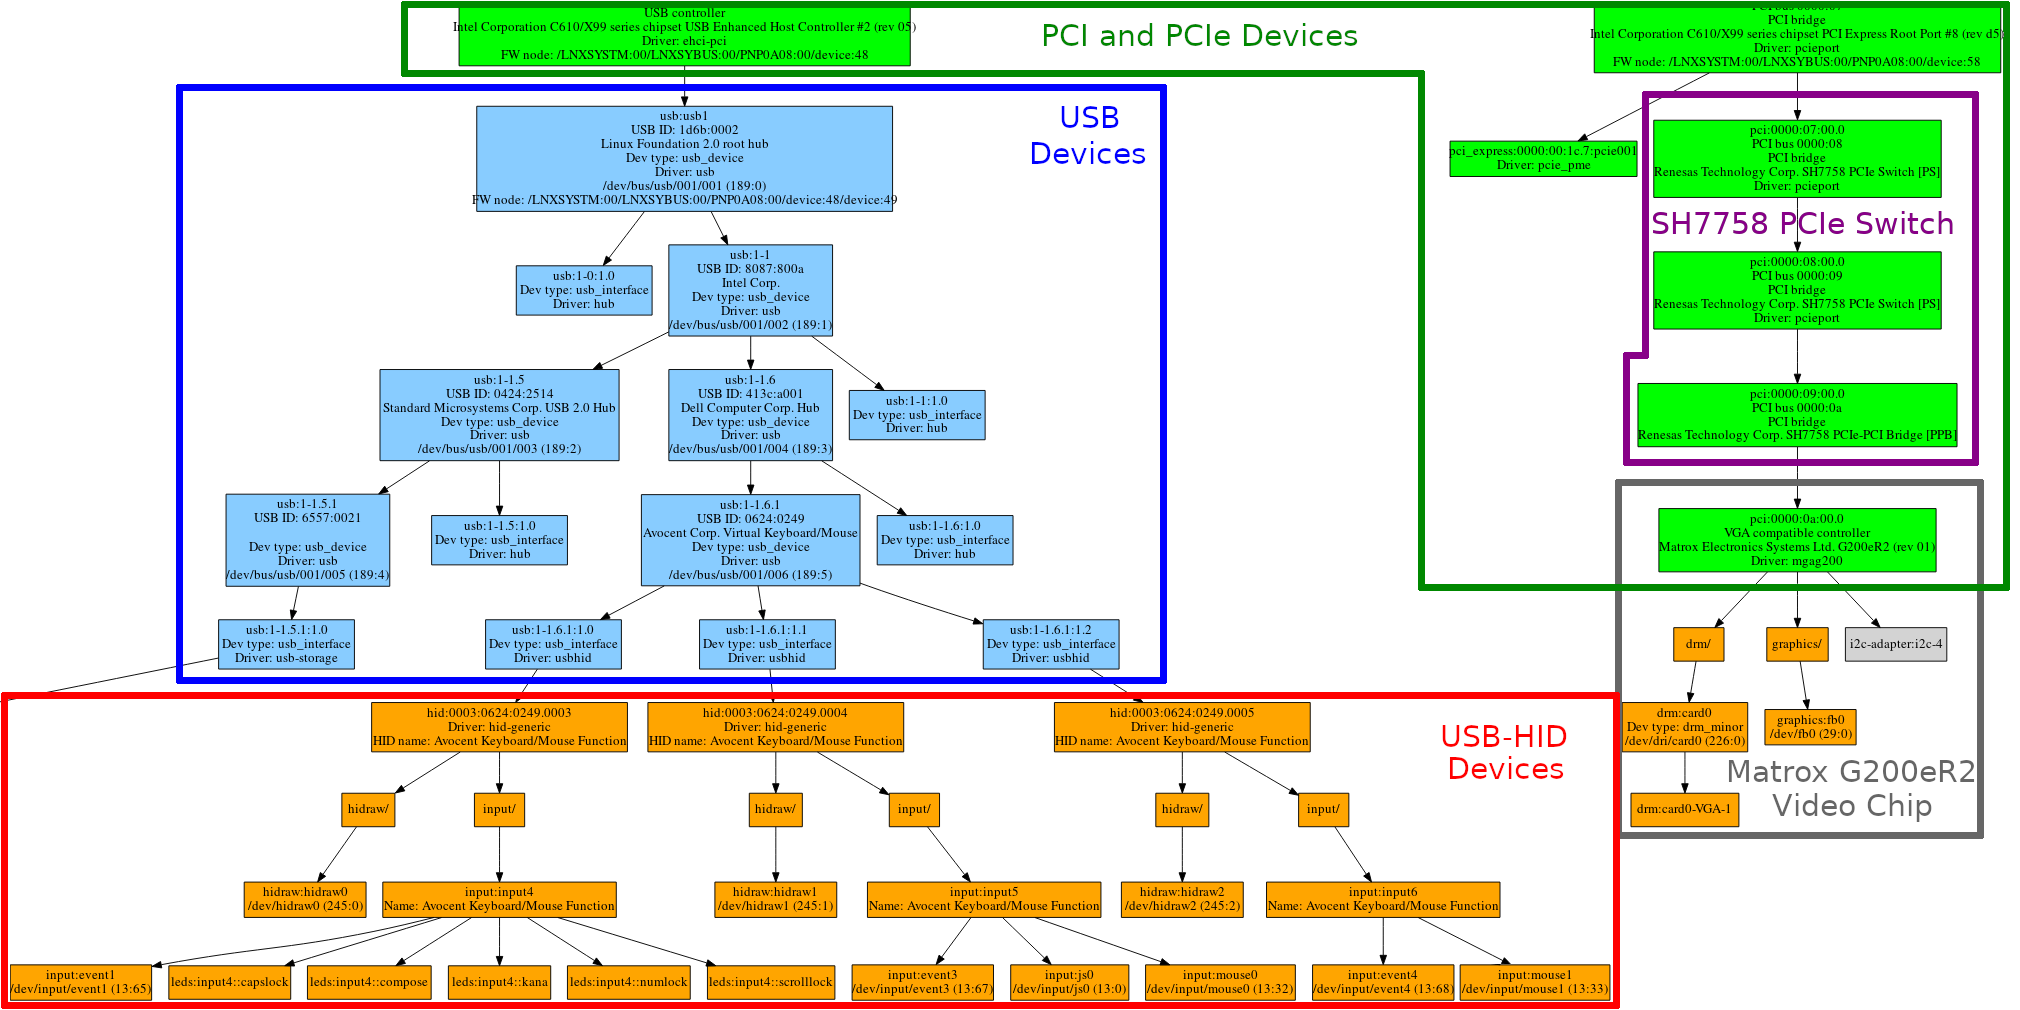
\includegraphics[height=.74\textwidth,angle=90,origin=c]{03-idrackar/img/graph-hw_usb_pci_host.png}
  \caption{Extract of device tree from the main operating system (green: PCIe devices, blue: USB devices, orange: HID and graphics devices, gray: I²C devices).}
  \label{fig:idrackar:graph-hw-main-linux}
\end{figure}

The main operating system communicates with the iDRAC using several channels provided by hardware components.
When the OS is Linux, the virtual filesystem in \texttt{/sys} gives detailed information about the available hardware.
With a tool such as \texttt{graph-hw}\footnote{\url{https://github.com/fishilico/home-files/blob/master/bin/graph-hw}} (which has already been presented at SSTIC\footnote{The rump session entitled \emph{Représenter l'arborescence matérielle} is available at \url{https://www.sstic.org/2018/presentation/2018_rumps/}.}), this information can be represented as a graph that is easier to analyze (figure~\ref{fig:idrackar:graph-hw-main-linux}).

The hardware peripherals that are exposed are the following ones:
\begin{itemize}
  \item USB-HID devices (keyboard, mouse) named ``Avocent Keyboard / Mouse Function'' connected to a USB hub named ``Dell Computer Corp. Hub'', itself connected to a USB hub from Intel that is connected to a USB controller.
    Moreover, when a USB device is connected to the front panel of the studied Dell server, it appears below the same Intel USB hub.
    This makes it likely for this hub to be a real device in the server.
    The iDRAC then uses real USB connectivity to connect its virtual keyboard and mouse to the hardware tree of the main operating system\footnote{This is major difference between Dell iDRAC and HP iLO4, as the later implements a virtual USB controller in its firmware.}.
  \item The graphics card (a Matrox G200eR2 identified thanks to device nodes \texttt{/dev/fb0} and \texttt{/dev/dri/card0} on the right part of figure~\ref{fig:idrackar:graph-hw-main-linux}) is accessed through a chain of PCI switches and bridges.
    Several of these devices are named ``Renesas [...] SH7758'' (figure~\ref{fig:idrackar:pcie-device-ids}), which is the name of the CPU used by the iDRAC.
    This could mean that the iDRAC CPU has direct access to the PCIe bus.

  \item The Linux kernel creates a device node named \texttt{/dev/ipmi0} which can be used to issue IPMI commands to the iDRAC.
    The driver stack of this device uses kernel modules \texttt{ipmi\_devintf}, \texttt{ipmi\_si}, \texttt{ipmi\_ssif} and \texttt{ipmi\_msghandler} in order to transmit and receive IPMI messages over the SMBus (System Management Bus) with protocols such as KCS (Keyboard-Controller Style), SMIC (System Management Interface Chip) or BT (Block Transfer).
\end{itemize}

\begin{figure}[ht]
  \begin{tabular}{|>{\tt}c|>{\tt}c|l|l|}
    \hline
    \bf Vendor ID & \bf Device ID & \multicolumn{1}{c|}{\bf Vendor name} & \multicolumn{1}{c|}{\bf Device name} \\
    \hline
    \multirow{2}{*}{8086} & \multirow{2}{*}{8d1e} & \multirow{2}{*}{Intel Corporation} & C610/X99 series chipset PCI \\
         &      & & Express Root Port \#8 \\
    \hline
    1912 & 001d & Renesas Technology Corp. & SH7758 PCIe Switch [PS] \\
    \hline
    1912 & 001a & Renesas Technology Corp. & SH7758 PCIe-PCI Bridge [PPB] \\
    \hline
    \multirow{2}{*}{102b} & \multirow{2}{*}{0534} & Matrox Electronics & \multirow{2}{*}{G200eR2} \\
         &      &  Systems Ltd. & \\
    \hline
  \end{tabular}
  \caption{Table of PCIe device identifiers on the path to the graphics card, as seen from the main operating system.}
  \label{fig:idrackar:pcie-device-ids}
\end{figure}

More interfaces between the iDRAC and the main operating system might exist and might be more difficult to discover.
Focusing on the interfaces that were enumerated, how are they used by iDRAC's firmware?

\subsection{The hardware seen from the iDRAC}

As iDRAC's firmware has been build from Linux, information about the hardware accessible from the iDRAC can be gathered by browsing \texttt{/dev} and \texttt{/sys}, reading kernel logs and \texttt{/proc/iomem}, etc.
Moreover, the firmware uses custom kernel modules, which source files are freely available on \url{https://opensource.dell.com/}.
These source files allow getting a better understanding of hardware components.

First, iDRAC's firmware does not see any PCI device tree: there is neither \texttt{/sys/bus/pci/} nor any PCI device in \texttt{/sys/devices/}.
There exists nevertheless a USB Device Controller (UDC) named ``R8A66597''.
This controller exposes several USB gadget devices (figure~\ref{fig:idrackar:idrac-usb-devices}).

\begin{figure}[ht]
  \centering
  \vspace*{-.2cm}
  \begin{tabular}{|c|c|l|}
    \hline
    \bf Directory name in & \multirow{2}{*}{\bf Driver name} & \multicolumn{1}{c|}{\multirow{2}{*}{\bf Device nodes}} \\
    \texttt{/sys/devices/platform/} & & \\
    \hline
    \texttt{r8a66597\_udc.0} & \texttt{g\_hub} & \\
    \hline
    \texttt{r8a66597\_udc.1} & \texttt{g\_kbdmouse} & \texttt{/dev/avct/usb\_keyboard} \\
    & & \texttt{/dev/avct/usb\_mouse} \\
    \hline
    \texttt{r8a66597\_udc.2} & \texttt{g\_mass\_storage} & \texttt{/dev/avct/usb\_iface1} \\
    \hline
    \texttt{r8a66597\_udc.3} & & \\
    \hline
    \texttt{r8a66597\_udc.4} & \texttt{g\_mass\_storage1} & \texttt{/dev/avct/usb\_iface2} \\
    \hline
    \texttt{r8a66597\_udc.5} & \texttt{g\_mass\_storage2} & \texttt{/dev/avct/usb\_iface3} \\
    \hline
    \texttt{r8a66597\_udc.6} & \texttt{g\_mass\_storage3} & \texttt{/dev/avct/usb\_iface4} \\
    \hline
    \texttt{r8a66597\_udc.7} & \texttt{g\_ether} & network interface \texttt{usb1} \\
    \hline
  \end{tabular}
  \vspace*{-.2cm}
  \caption{Table of USB gadget devices used by iDRAC's R8A66597 UDC.}
  \vspace*{-.3cm}
  \label{fig:idrackar:idrac-usb-devices}
\end{figure}

The USB keyboard and mouse match the USB devices that were seen from the main operating system.
The mass storage USB devices can appear on the main operating system when a user enables a virtual CDROM or a virtual Floppy in the remote console.
The Ethernet network interface was not present in USB devices from the main operating system.
Nevertheless, by investigating the available commands on the iDRAC, it appears that it is possible to enable this interface with a command accessible from iDRAC's shell (SHASH CLP), using a subcommand named ``\texttt{racadm}'' (listing~\ref{lst:idrackar:pop-net}).
The network interface will then appear on the main operating system as an Ethernet-over-USB interface next to the keyboard/mouse USB device.
On systems running systemd, this interface is named \texttt{idrac} and can be configured like usual network interfaces.
Researchers from Immunity, Inc. found that this command can also be used from the main operating system, through the IPMI channel~\cite{idrackar:bhus2018bmc}.

\begin{lstlisting}[language={},caption={Enabling a network interface from iDRAC's shell.},label={lst:idrackar:pop-net}]
[SH7757 /flash/data0/home/root]$ clpd
/admin1-> racadm get iDRAC.OS-BMC
[Key=iDRAC.Embedded.1#OS-BMC.1]
AdminState=Disabled
OSIpAddress=0.0.0.0
#PTCapability=Capable
PTMode=usb-p2p
UsbNicIpAddress=169.254.0.1

/admin1-> racadm set iDRAC.OS-BMC.AdminState Enabled
[Key=iDRAC.Embedded.1#OS-BMC.1]
Object value modified successfully
\end{lstlisting}

The server graphics card does not seem to be accessible in usual ways from the iDRAC, as the filesystem does not show \texttt{/dev/dri/} nor \texttt{/dev/fb0} nor \texttt{/sys/class/drm/}.
However, \texttt{/proc/iomem} contains some entries that refer to a video device (listing~\ref{lst:idrackar:proc-iomem-video}).

\begin{lstlisting}[language={},caption={Entries related to video in \texttt{/proc/iomem}.},label={lst:idrackar:proc-iomem-video}]
[SH7757 /flash/data0/home/root]$ grep video /proc/iomem
fe900000-fe90003b : aess_video
fea02000-fea02fff : aess_video
ff000030-ff000047 : aess_video
ffc10000-ffc1013f : aess_video
\end{lstlisting}

There also exist some special files related to the video device:
\begin{itemize}
  \item \texttt{/dev/avct/video} is a character device with major number 253 and minor number 0. \texttt{/proc/devices} tells that this device is handled by a kernel module named \texttt{aess\_video}.
  \item \texttt{/proc/aess\_video} gives some information about a video device (memory addresses, checksums, etc.).
\end{itemize}

The source code of \texttt{aess\_video}\footnote{The \texttt{externalsrc/linux-drivers/video\_driver} directory comes from archives downloaded from \url{https://opensource.dell.com/}.} contains some comments that describe the role of the memory regions identified in \texttt{/proc/iomem} (listing~\ref{lst:idrackar:aess-video-comments}).


\begin{lstlisting}[language={C},caption={\texttt{externalsrc/linux-drivers/video\_driver/aess\_video.h}.},label={lst:idrackar:aess-video-comments}]
/*
 * DVC5 register base addres
 */
#define PBASE_DVC5_ADDR 0xFEA02000
#define VIDEO_CORE_REG_SIZE 0x1000

/*
 * Graphic controller register base address
 */
#define PBASE_GCTRL_ADDR 0xFFC10000
#define GCTRL_REG_SIZE 0x140

/*
 * ECD register base address
 */
#define PBASE_ECD_ADDR 0xFE900000
#define ECD_REG_SIZE 0x3C

/*
 * SH7757 Version and Product registers
 */
#define PBASE_VERSION_ADDR 0xFF000030
#define VERSION_REG_SIZE 0x18
\end{lstlisting}

This kernel module uses components that are named with acronyms that do not have a clear definition: ``DVC Engine'' and ``ECD/ECC''.
``DVC'' is also used in a function comment in another file, to describe a video file format (listing~\ref{lst:idrackar:librpipc-comments}).
This function does not seem to be used anywhere in iDRAC's firmware, but a function nearby, named \texttt{avct\_vkvm\_capture\_screen} is directly usable through command \texttt{avct\_control} in order to take a screenshot in PNG format (listing~\ref{lst:idrackar:ssh-screenshot}).
Using \texttt{strace} in order to understand how \texttt{avct\_control} interacts with the screen, it is observed that the only relevant operations that \texttt{avct\_control} does consists in sending a message to \texttt{/sbin/avct\_server} over a Unix socket located in \texttt{/tmp/rpSocket}.

\begin{lstlisting}[language={C},caption={Extract from header file \texttt{ipk-dropbox/librpipc/image/usr/ include/librpipc/avct/rpipc.h}.},label={lst:idrackar:librpipc-comments}]
/*!
 *  Description: Start capture of host video in DVC format to the specified file.
 *
 * szName - The file name (including path) to store the file to.
 * ulSize - The maximum size for the video file.
 */
int avct_vkvm_start_video_capture(const char *szName, uint32_t ulSize);
\end{lstlisting}

\begin{lstlisting}[language={},caption={Screenshot from iDRAC's SSH.},label={lst:idrackar:ssh-screenshot}]
[SH7757 /dev/shm]$ avct_control --file $(pwd)/my-screen.png capture
Capturing screen to file '/dev/shm/my-screen.png'...
Captured.
[SH7757 /dev/shm]$ hd < /dev/shm/my-screen.png
00000000 89504e470d0a1a0a 0000000d49484452  |.PNG........IHDR|
00000010 0000050000000400 080200000031f163  |.............1.c|
00000020 1400002000494441 547801eddd4192a3  |... .IDATx...A..|
00000030 b8120050bba3161c 8fa58fe825c7f3f2  |...P........%...|
...
\end{lstlisting}

In the end, the iDRAC does not use the PCIe bus in order to interact with the graphics card but uses specific components to retrieve the content of the screen.

%\todo{IPMI /dev/ipmi0 from iDRAC? With program fullfw?}

\subsection{The CPLD, a large GPIO device}

Several files, programs and libraries on the iDRAC refer to a CPLD\footnote{Complex Programmable Logic Device. On the studied server, it is an Intel Altera MAX II whose part number is EPM2210F324C5N.}, a programmable logic device that can be used to implement features and algorithms without manufacturing a custom chipset.
Such a device might be used to implement a PCIe endpoint, which is why studying its use on iDRAC is interesting.

iDRAC 8's CPLD can be used by programs through a library, \texttt{/usr/lib/libcpld.so.1.2.3}, which uses a character device node, \texttt{/dev/dell\_cplddrv}, to get and set bits in the CPLD.
The operations on this node are implemented by a kernel module named \texttt{dell\_cplddrv.ko}, which source code is available on \url{https://opensource.dell.com/}.
The code contains some references to USB removable events (cf. listing~\ref{lst:idrackar:cplddrv-usb}).

\begin{lstlisting}[language={C},caption={Extract of the \texttt{cpldisr\_13g} function, from file \texttt{externalsrc/linux-drivers/cpld\_driver/dell\_cplddrv.c}.},label={lst:idrackar:cplddrv-usb}]
    /* save interrupt cause for user retrieval */
    intrcause = (cpld_read(0x10)&0xf);  //ID Button latch
    if(intrcause & ID_LATCH_MASK){
        cpld_rmw(ID_LATCH_MASK, ID_LATCH_MASK, 0x10);  //clear interrupt
    }
/* ... */
    /* Check if the CPLD 0x14000019 Bit 1 is Asserted  */
    if( USB_REMOVAL_MASK == (cpld_read(0x19) & USB_REMOVAL_MASK) )
    {
        cpld_rmw(CPLD_USB_PCH_REMOVAL_MASK,
            CPLD_USB_PCH_REMOVAL_MASK,CPLD_USB_CONFIG_OFFSET); //clear interrupt
        intrcause |=CPLD_INT_PCH_USB_REMOVE;
        up(&pchusb_removal_sem);
    }
\end{lstlisting}

Some bits of the CPLD are used by the iDRAC to read the state of the ``ID button'' of the server.
Others are used to connect and disconnect virtual USB devices such as the mouse and keyboard used by the virtual console.
The analysis of the use of the CPLD gives the impression that it behaves like GPIO devices: each bit has a specific meaning and can be used as an boolean input/output interface.
It seems therefore unlikely for iDRAC's CPLD to provide a way to access the main memory of the server.
Moreover, some architecture diagrams (figure~\ref{fig:idrackar:idrac-hardware-diagram}) shows the CPLD device as being in the opposite side to the buses between the iDRAC and the main CPU.
This makes it difficult for the CPLD to be a way to reach the main memory from the iDRAC.


\subsection{The mysterious PBI device}

When looking for data about the PCIe bridges that were seen between the PCIe root complex and the graphics card (section~\ref{sect:idrackar:hardware-from-os}), several search engines give pages on Ubuntu Certified hardware's website\footnote{\url{https://certification.ubuntu.com/}}.
For example \url{https://certification.ubuntu.com/catalog/component/pci/1912%3A001d/} gives a list of Dell servers that share a ``Renesas Technology Corp. SH7758 PCIe Switch [PS]''.

\begin{figure}[ht]
  \centering
  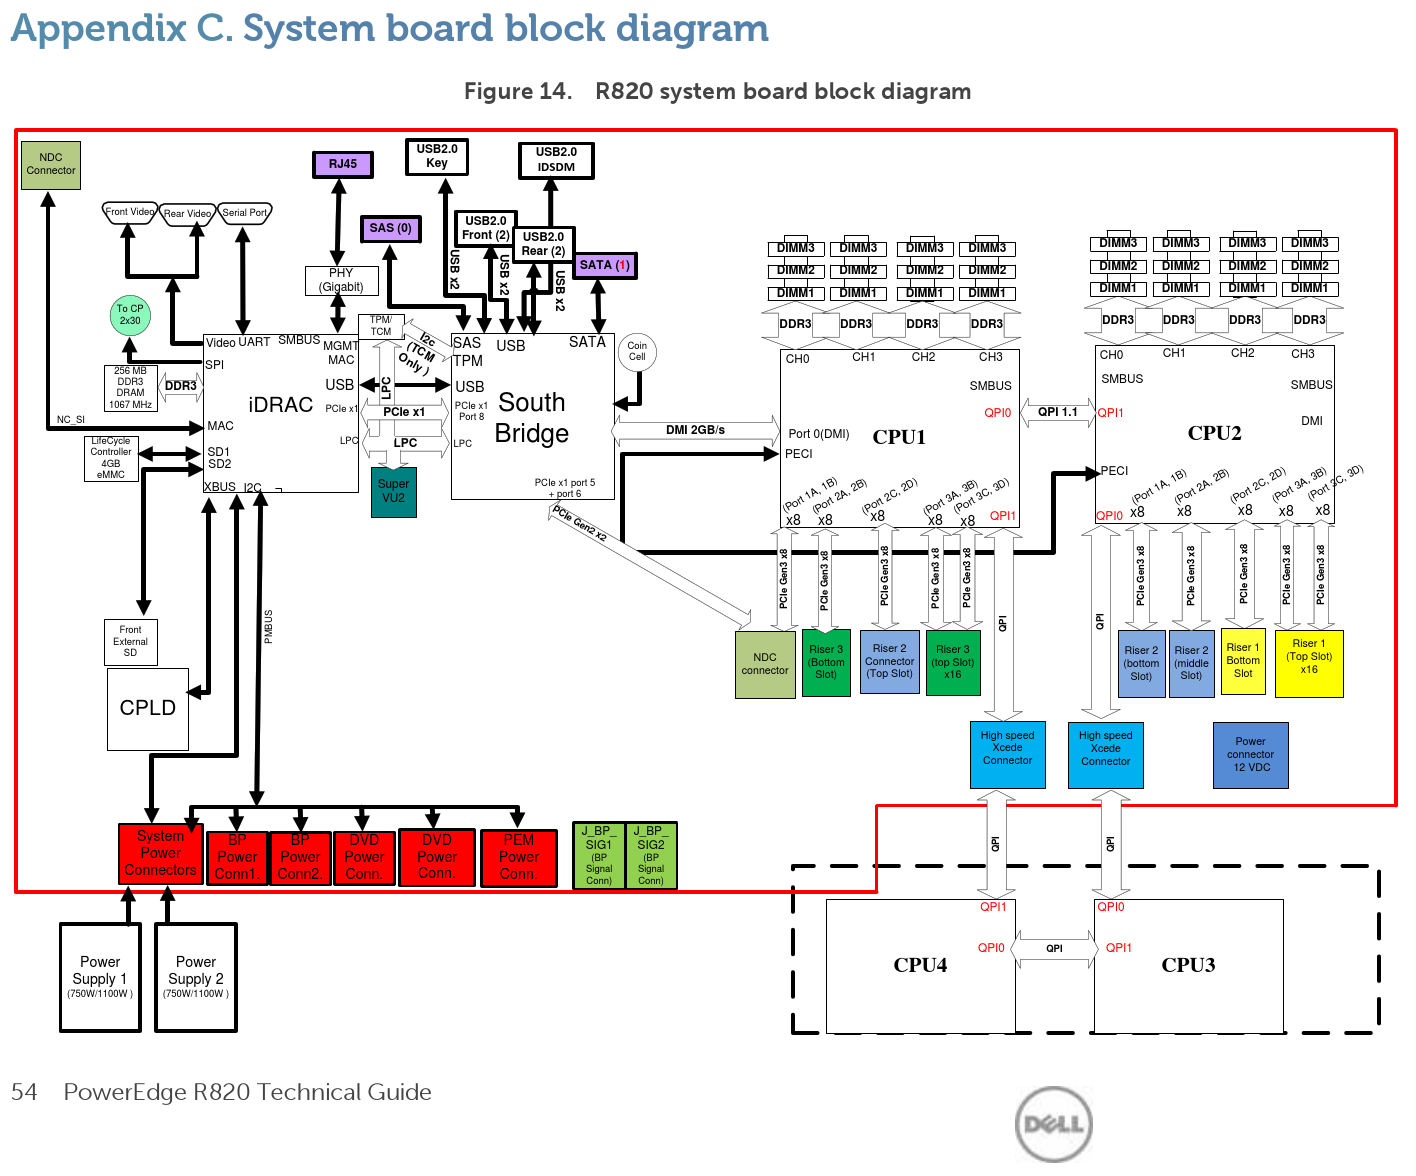
\includegraphics[width=\textwidth]{03-idrackar/img/dell-poweredge-r820-hw.png}
  \caption{Diagram of iDRAC hardware.}
  \label{fig:idrackar:idrac-hardware-diagram}
  {\scriptsize Source: \url{https://www.manualslib.com/manual/624251/Dell-Poweredge-R820.html?page=54}}\vspace*{-.3cm} % Don't do this at home!
\end{figure}

Another page, \url{https://certification.ubuntu.com/catalog/component/pci/1912%3A001b/} gives a list of servers that has a PCIe endpoint device named ``Renesas Technology Corp. SH7758 PCIe End-Point [PBI]''.
This device does not seem to exist on the studied Dell PowerEdge R730 server, but a kernel module in the firmware refers to it.
In the files downloaded from \url{https://opensource.dell.com/}, directory \texttt{externalsrc/linux-drivers/pbi\_driver/} contains the source code of a module described as ``Linux driver for PBI shared memory and mailbox FIFO on the Renesas SH7757 iBMC Controller''.
This module uses hardware registers which are mapped at addresses \texttt{0xffca0000} and \texttt{0xffcaa000}.
These addresses are invisible from \texttt{/proc/iomem}, but this does not mean that the studied iDRAC system does not support this device.
Searching for these addresses through iDRAC's firmware leads to functions in U-Boot and Linux (listings~\ref{lst:idrackar:u-boot-init-mailbox} and~\ref{lst:idrackar:linux-pcie-shared}).

\begin{lstlisting}[language={C},caption={Extract from U-Boot's function \texttt{init\_mailbox}, in \texttt{externalsrc/ u-boot-idrac8/u-boot\_B0/board/renesas/sh7757lcr/util\_idrac\_main.c}.},label={lst:idrackar:u-boot-init-mailbox}]
HAL_writel(0x1, 0xffca1420);  //PCIE_BARMAP0, Mailbox BAR Mapping
HAL_writel(0x4, 0xffca1470);  //PCIE_PBICTL2, A Reserved Bit??>
HAL_writel(0x0, 0xffca1604);  //PCIE_BSTCTL0, Disable Burst Xfer
HAL_writel(0x30000, 0xffca160c); //PCIE_ENDICTL0
HAL_writel(0x3, 0xffca1610);  //PCIE_ENDICTL1

HAL_writel(0xffcaa000, 0xffca1260); //PCIE_LAD0, Local Address Register 0 
HAL_writel(0xff2, 0xffca1264); //PCIE_LADMSK0, Local Address Mask Register 0 
HAL_writel(0xe500e000, 0xffca1268); //PCIE_LAD1
HAL_writel(0x72, 0xffca126c);       //PCIE_LADMSK1
/* ... */
/* 
 * DF533855 PCIe Training fix.  I have no idea what this is/does.
 * Renesas says to put it in.
 */
*(u32*)0xFFEE0150 = 0x40010000;

snprintf(msg, MAX_MSG_LEN, "Init PCIe mailbox(PCIe 0xFFEE0150=0x40010000)");
\end{lstlisting}

\begin{lstlisting}[language={C},caption={Extract from Dell's Linux source tree, in \texttt{externalsrc/ linux-yocto/arch/sh/boards/board-sh7757lcr.c}.},label={lst:idrackar:linux-pcie-shared}]
#define PCIE_BASE   0xffca0000
#define LADMSK0     (PCIE_BASE + 0x1264)
#define BARMAP      (PCIE_BASE + 0x1420)

static int __init sh_pcie_init(void)
{
    printk(KERN_INFO "enable PCIe shared memory area\n");

    __raw_writel(0x00000ff2, LADMSK0);
    __raw_writel(0x00000001, BARMAP);

    return 0;
}
\end{lstlisting}

In order to read the current configuration of these hardware registers, it would be possible to craft a program that opens \texttt{/dev/mem} and reads data from iDRAC's physical memory.
This is nevertheless not needed as Dell provides two programs that can be used to access this memory: \texttt{MemAccess} and \texttt{MemAccess2} (listing~\ref{lst:idrackar:memaccess-pbi}).

\begin{lstlisting}[language={},caption={Using \texttt{MemAccess2} to read PBI's PCIe configuration.},label={lst:idrackar:memaccess-pbi}]
[SH7757 /]$ MemAccess2 -rl -a ffca0000
0xffca0000 = 001b1912 00100007 : 05000000 00000000
0xffca0010 = 91901000 91900000 : 00000000 00000000
0xffca0020 *
0xffca0030 = 00000000 00000040 : 00000000 000001ff
\end{lstlisting}

Using \texttt{lspci} on another computer to decode the dumped data leads to an output that seems reasonable for PCIe configuration registers (listing~\ref{lst:idrackar:lspci-pbi}).

\begin{lstlisting}[language={},caption={Parsing of PBI's PCIe configuration with \texttt{lspci}.},label={lst:idrackar:lspci-pbi}]
$ lspci -nnvvvxxx -F pbi-config-dump.hex
RAM memory [0500]: Renesas Technology Corp. SH7758 PCIe End-Point [PBI] [1912:001b]
    Control: I/O+ Mem+ BusMaster+ SpecCycle- MemWINV- VGASnoop- ParErr- Stepping- SERR- FastB2B- DisINTx-
    Status: Cap+ 66MHz- UDF- FastB2B- ParErr- DEVSEL=fast >TAbort- <TAbort- <MAbort- >SERR- <PERR- INTx-
    Latency: 0
    Interrupt: pin A routed to IRQ 255
    Region 0: Memory at 91901000 (32-bit, non-prefetchable)
    Region 1: Memory at 91900000 (32-bit, non-prefetchable)
    Capabilities: [40] Power Management version 3
        Flags: PMEClk- DSI- D1- D2- AuxCurrent=0mA PME(D0-,D1-,D2-,D3hot+,D3cold-)
        Status: D0 NoSoftRst+ PME-Enable- DSel=0 DScale=0 PME-
    Capabilities: [50] MSI: Enable- Count=1/8 Maskable- 64bit+
        Address: 0000000000000000  Data: 0000
    Capabilities: [70] Express (v2) Endpoint, MSI 07
        DevCap: MaxPayload 128 bytes, PhantFunc 0, Latency L0s <64ns, L1 <1us
            ExtTag+ AttnBtn- AttnInd- PwrInd- RBE+ FLReset+ SlotPowerLimit 0.000W
        DevCtl: Report errors: Correctable- Non-Fatal+ Fatal+ Unsupported+
            RlxdOrd+ ExtTag+ PhantFunc- AuxPwr- NoSnoop+ FLReset-
            MaxPayload 128 bytes, MaxReadReq 4096 bytes
        DevSta: CorrErr- UncorrErr- FatalErr- UnsuppReq- AuxPwr- TransPend-
        LnkCap: Port #0, Speed 2.5GT/s, Width x1, ASPM L0s, Exit Latency L0s unlimited
            ClockPM- Surprise- LLActRep- BwNot- ASPMOptComp+
        LnkCtl: ASPM Disabled; RCB 64 bytes Disabled- CommClk-
            ExtSynch- ClockPM- AutWidDis- BWInt- AutBWInt-
        LnkSta: Speed 2.5GT/s, Width x1, TrErr- Train- SlotClk- DLActive- BWMgmt- ABWMgmt-
        DevCap2: Completion Timeout: Not Supported, TimeoutDis+, LTR-, OBFF Not Supported
        DevCtl2: Completion Timeout: 50us to 50ms, TimeoutDis-, LTR-, OBFF Disabled
             AtomicOpsCtl: ReqEn-
        LnkCtl2: Target Link Speed: 2.5GT/s, EnterCompliance- SpeedDis-
             Transmit Margin: Normal Operating Range, EnterModifiedCompliance- ComplianceSOS-
             Compliance De-emphasis: -6dB
        LnkSta2: Current De-emphasis Level: -6dB, EqualizationComplete-, EqualizationPhase1-
             EqualizationPhase2-, EqualizationPhase3-, LinkEqualizationRequest-
00: 12 19 1b 00 07 00 10 00 00 00 00 05 00 00 00 00
10: 00 10 90 91 00 00 90 91 00 00 00 00 00 00 00 00
20: 00 00 00 00 00 00 00 00 00 00 00 00 00 00 00 00
30: 00 00 00 00 40 00 00 00 00 00 00 00 ff 01 00 00
40: 01 50 03 40 08 00 00 00 00 00 00 00 00 00 00 00
50: 05 70 86 00 00 00 00 00 00 00 00 00 00 00 00 00
60: 00 00 00 00 00 00 00 00 00 00 00 00 00 00 00 00
70: 10 00 02 0e 20 80 00 10 1e 59 00 00 11 f4 43 00
80: 00 00 11 00 00 00 00 00 00 00 00 00 00 00 00 00
90: 00 00 00 00 10 00 00 00 00 00 00 00 00 00 00 00
a0: 00 00 00 00 00 00 00 00 00 00 00 00 00 00 00 00
b0: 00 00 00 00 00 00 00 00 00 00 00 00 00 00 00 00
c0: 00 00 00 00 00 00 00 00 00 00 00 00 00 00 00 00
d0: 00 00 00 00 00 00 00 00 00 00 00 00 00 00 00 00
e0: 00 00 00 00 00 00 00 00 00 00 00 00 00 00 00 00
f0: 00 00 00 00 00 00 00 00 00 00 00 00 00 00 00 00
\end{lstlisting}

PBI's kernel module creates device node \texttt{/dev/sh\_pbi}, which can be used by iDRAC's userspace programs.
iDRAC's firmware contains command \texttt{pbitest} and library \texttt{libpbidrv.so} that use this device in order to communicate with something unknown using a \emph{mailbox}.
After reading the content of \texttt{lib\_pbidrv.h}, it appears that the PBI is used as a communication channel between the main operating system and the iDRAC in order to control the LCD screen that may be found on the front panel of a server: this LCD is managed by the iDRAC and the main operating system can issue commands to make the iDRAC perform some actions on it (display a text, read the state of its buttons, etc.).

Looking back at these findings, something seems missing: this PBI device does not appear in the PCIe device tree of the main operating system of the studied server, even though it is possible for the main operating system to control the content of the LCD.
Reading more web pages leads to several scripts and a Dell document named ``Using IPMItool raw commands for remote management of dell PowerEdge Servers''\footnote{\url{https://www.dell.com/downloads/global/power/ps4q07-20070387-Babu.pdf}}.
This document gives two \texttt{ipmitool} commands to write custom messages on the LCD display (listing~\ref{lst:idrackar:ipmitool-lcd}).
\texttt{ipmitool} sends IPMI commands to the iDRAC through the SMBus or through the network, not through the PCIe bus.

\begin{lstlisting}[language={},caption={Create custom LCD messages with IPMItool.},label={lst:idrackar:ipmitool-lcd}]
ipmitool raw 0x6 0x58 193 0 0 length ASCII_hex_values
ipmitool raw 0x6 0x58 194 0
\end{lstlisting}

Even though using a PCIe device such as the PBI is not needed to allow the main operating system to define messages displayed on the LCD display of the server, the PBI still exists.
Its PCIe configuration registers are present in iDRAC's physical memory but the device seems to be somehow disabled.
A comment in U-Boot's source code clarifies the situation: Dell configured the device to be ``hidden'' (listing~\ref{lst:idrackar:uboot-hide-pbi}).

{\captionsetup{margin=4.5pt,font=footnotesize,labelfont=bf,labelsep=period}
\begin{lstlisting}[language={C},caption={Extract from U-Boot's \texttt{init\_pcie\_bridge} function, in \texttt{externalsrc/u-boot-idrac8/u-boot\_B0/board/renesas/sh7757lcr/sh7757lcr.c}.},label={lst:idrackar:uboot-hide-pbi}]
    // On 13G systems, fix issue with hiding PBI device. Writing to PSPPBCTL DRS[1:0] = '01b'
    if(is_sh7758())
            writel(0x00000100, 0xffd60080);
\end{lstlisting}}

As hiding the device is performed by setting a bit to 1 in a 32-bit value at \texttt{0xffd60080} (in iDRAC's physical memory), setting this bit to zero might unhide it.
Unfortunately, doing \texttt{MemAccess2 -wl -a ffd60080 -d 00000000} to clear the bit leads to a freeze of the main operating system, which is then unable to boot (the screen stays black).
Setting the bit back to one (with \texttt{MemAccess2 -wl -a ffd60080 -d 00000100}) makes the main operating system boot again.
This might be an issue that Dell experienced which led to the hiding of the PBI device on 13th Generation servers (using iDRAC 8).

To conclude this part, iDRAC 8's firmware contains code for a hidden PCIe device named PBI.
It is possible that this device was used to allow the main operating system to define the content of the LCD display of the server, but in iDRAC 8 there exists another way to perform this operation, through IPMI commands.
The code hiding the PBI modifies a register of a component named ``PCIe bridge'' in U-Boot's code.
The next part focuses on this component.

\subsection{The mythical PCIe bridge's microcode}

While looking at references to the PCIe bus in Dell's U-Boot code, several parts refer to a PCIe bridge.
For example, \texttt{externalsrc/u-boot-idrac8/u-boot\_B0/board/renesas/sh7757lcr/ bld\_bridge.c} defines a \emph{usage} function which prints:
\begin{quote}
  {\footnotesize
  \texttt{Usage: bld\_bridge <pcie\_bridge.src> <7757|7758> <util\_pciebridge775X.c>}}
\end{quote}

\noindent
This file also contains a comment from Dell's developers:
\begin{quote}
  \footnotesize
  The PCIe section of the Renesas processor requires u-boot to load the PCIe
  microcode.  Renesas uses a dedicated sector/s to store this info.  Dell
  cannot leave this as a seperate sectors because the versioning and test
  matrix make this a big mess.  So we will make it part of u-boot.
\end{quote}

The function that loads this PCIe microcode is \texttt{init\_pcie\_bridge}, located in \texttt{sh7757lcr.c} (listing~\ref{lst:idrackar:u-boot-pcie-bridge-init}).
It uses four hardware registers:
\begin{itemize}
  \item \texttt{PCIEBRG\_CTRL\_H8S = 0xffd60000} in order to reset and start the PCIe bridge controller~;
  \item \texttt{PCIEBRG\_CP\_ADDR = 0xffd60010} in order to configure the start address of the loaded microcode (\texttt{0x0000})~;
  \item \texttt{PCIEBRG\_CP\_DATA = 0xffd60014} in order to load the microcode by chunks of 16 bits~;
  \item \texttt{PCIEBRG\_CP\_CTRL = 0xffd60018}.
\end{itemize}

{\captionsetup{margin=4.5pt,font=footnotesize,labelfont=bf,labelsep=period}
\begin{lstlisting}[language={C},caption={Extract from U-Boot's \texttt{init\_pcie\_bridge} function, in \texttt{externalsrc/u-boot-idrac8/u-boot\_B0/board/renesas/sh7757lcr/sh7757lcr.c}.},label={lst:idrackar:u-boot-pcie-bridge-init}]
writew(0xa501, PCIEBRG_CTRL_H8S);  /* reset */
writew(0x0000, PCIEBRG_CP_CTRL);
writew(0x0000, PCIEBRG_CP_ADDR);
for (i = 0; i < pcie_cnt; i += 2) {
    tmp = (data[i] << 8) | data[i + 1];
    writew(tmp, PCIEBRG_CP_DATA);
}
writew(0xa500, PCIEBRG_CTRL_H8S);  /* start */
if (!is_sh7757_b0())  /* Cn or Shasta */
    writel(0x00000001, PCIE_PBICTL3);  /* PBI control register3 */
\end{lstlisting}}

The microcode which is loaded can be found in the archive published on \url{https://opensource.dell.com/} next to U-Boot's code.
It indeed comes from either \texttt{bridge7757.mot} or \texttt{bridge7758.mot}, which are files in Motorola S-Record format.
The files can be converted into raw binary files using a command such as \texttt{objcopy -I srec -O binary input-file.mot output-file}.
In order to find out which file is used on the studied Dell PowerEdge R730 server, a possible way consists in reading U-Boot's log using ``\texttt{dellutil ublog}'' from iDRAC's shell  (listing~\ref{lst:idrackar:dellutil-ublog}).
As this log contains ``\texttt{SH7758\_A0}'', \texttt{bridge7758.mot} contains the loaded microcode.

\begin{lstlisting}[language={},caption={Extract from command \texttt{dellutil ublog}.},label={lst:idrackar:dellutil-ublog}]
$ dellutil ublog
INFO: 00:007 SH-4A Product: Major Ver=0x31  Minor Ver=0x20 D0 Little endian
             Family=0x10    Major Ver=0x30  Minor Ver=0x0b
...
PASS: 00:008 PCIe SH7758_A0 Ver=0.03 MCTP en, CRC=0x70ae6992 @0x8efd591c cnt=0x18000
INFO: 00:008 Init PCIe mailbox(PCIe 0xFFEE0150=0x40010000)
\end{lstlisting}

The binary content of the microcode starts with a kind of header which is parsed using \texttt{struct pcie\_brg\_hdr} in \texttt{util\_idrac\_main.c}, followed by some data that starts at offset \texttt{0x100}.
This data does not look random enough to be compressed or encrypted.
The repetitions of 16-bit patterns suggests that this data contains code for a CPU using a 16-bit instruction set, which is neither x86 nor SH4.
Looking back at the code from \texttt{sh7757lcr.c} (listing~\ref{lst:idrackar:u-boot-pcie-bridge-init}), it appears that H8S is the name of a 16-bit microcontroller series made by Renesas.
It belongs to the H8 family, which also includes the 8-bit H8/300 microcontroller used in LEGO Mindstorms's RCX programmable brick.

Hex-Rays' interactive disassembler (IDA) supports many instruction sets from the H8 family, including ``Hitachi H8S advanced''.
This enables to confirm that the loaded microcode contains code at offset \texttt{0x100}.
Further analysis gives the following map of \texttt{bridge7758.mot}'s decoded content:
\begin{itemize}
  \item \texttt{0x0000} to \texttt{0x003b}: firmware header (listing~\ref{lst:idrackar:bridge7758-header-hex}).
    \begin{itemize}
      \item \texttt{0x0000}: address of entry point or reset vector entry (\texttt{0x0100} as 32-bit Big Endian integer).
      \item \texttt{0x0004}: chip version, \texttt{0x03} for SH7758 A0 (it is \texttt{0x00} for SH7757 A0, \texttt{0x01} for SH7757 B0 and \texttt{0x02} for SH7757 C0).
      \item \texttt{0x0005}: chip slice, \texttt{0x00} .
      \item \texttt{0x0006}: firmware version, \texttt{0x03}.
      \item \texttt{0x0007}: MCTP (Management Component Transport Protocol) mode, \texttt{0x01} (enabled).
      \item \texttt{0x0030} to \texttt{0x003b}: probably an interrupt vector table, with three 32-bit addresses of functions (\texttt{0x010a}, \texttt{0x01f8}, \texttt{0x033c}).
    \end{itemize}
  \item \texttt{0x0100} to \texttt{0x03a9}: code segment using H8S instruction set.
    This segment implements interrupt handlers and a reset handler that resets the stack to \texttt{0x00ffc000} and calls a function located at \texttt{0x0001685a} in a loop.
    This function is most likely the \texttt{main} function of the firmware.
  \item \texttt{0x03aa} to \texttt{0x2105}: read-only data segment.
    This segment contains 16-bit words that match the PCI vendor ID and device ID of the PCIe bridges listed in figure~\ref{fig:idrackar:pcie-device-ids} (section~\ref{sect:idrackar:hardware-from-os}).
  \item \texttt{0x2106} to \texttt{0x16929}: code segment, in H8S instruction set.
    This segment implements most of the functions of the firmware.
  \item \texttt{0x1692a} to \texttt{0x017fff}: padding with zeros.
\end{itemize}

\begin{lstlisting}[language={},caption={Hexadecimal dump of \texttt{bridge7758.mot}'s header.},label={lst:idrackar:bridge7758-header-hex}]
0000: 0000 0100 0300 0301 0000 0000 0000 0000
0010: 0000 0000 0000 0000 0000 0000 0000 0000
0020: 0000 0000 0000 0000 0000 0000 0000 0000
0030: 0000 010a 0000 01f8 0000 033c 0000 0000
\end{lstlisting}

One of the first steps of the analysis of the firmware consists in finding out how the memory space of the H8S microcontroller is organized.
Studying the performed memory accesses leads to the following layout:
\begin{itemize}
  \item \texttt{0x000000} to \texttt{0x017fff}: loaded firmware (98304 bytes)
  \item \texttt{0xffa000} to \texttt{0xffc000}: RAM (8192 bytes, global variables and stack, which is decreasing from the top)
  \item \texttt{0xffc000} to \texttt{0xffffff}: memory-mapped input/output (many hardware registers)
\end{itemize}

The H8S microcontroller uses 24-bit addresses.
This makes it difficult to perform the analysis using usual software, as most of them either restrict the address space to 16 bits or to 32 bits.
For example Hex-Rays' IDA software extends 16-bit addresses to 32 bits when using processor ``Hitachi H8S advanced (h8s300a)'', which messes up with the references of data located in RAM and IO regions.
Thankfully, IDA's processor ``Hitachi H8/300H advanced (h8300a)'' extends 16-bit addresses to 24 bits, so this processor module can be used instead of H8S.

When reading the code of many functions of the firmware, a common pattern stands out: nearly all functions starts by setting a 16-bit variable at address \texttt{0xffa9be} to a constant value.
For example the function starting from \texttt{0x002106} sets this value to \texttt{0x64}, the one starting from \texttt{0x002156} to \texttt{0x65}, the one from \texttt{0x0021a4} to \texttt{0x66}, etc.
This seems to indicate a kind of \emph{unique function identifier}, which can help to produce traces when debugging the code.

The value of this global variable is only read in one function of the firmware: the one starting at \texttt{0x00010a}.
This function could be an interrupt handler (for example to handle a timer).
It starts by reading the least significant bit of the byte located at \texttt{0xffd033}.
If this bit is set, it resets it, reads a 16-bit integer from \texttt{0xffd034} and runs instructions depending on the value.
The function then writes a 16-bit integer to \texttt{0xffd022} that comes from the instructions that were executed.

In short, the interrupt handler at \texttt{0x00010a} parses a 16-bit operation code from a hardware register, performs the specified operation and writes the result to another hardware register.
Figure~\ref{fig:idrackar:h8s-debug-cmds} enumerates the possible commands.

Can the iDRAC issue commands to the H8S through these 16-bit opcodes?
The study of the use of the hardware register located in \texttt{0xffd000} leads to several facts:
\begin{enumerate}
  \item In several locations, the firmware sets \texttt{0xffd000} to value \texttt{0xa501} and register \texttt{sp} (the stack pointer) to \texttt{0xffc000}.
  \item The iDRAC resets the H8S microcontroller by setting \texttt{0xffd60000} (in iDRAC's physical memory) to value \texttt{0xa501} (cf. listing~\ref{lst:idrackar:u-boot-pcie-bridge-init}).
  \item \texttt{0xffd000} is next to the addresses used by the function at \texttt{0x00010a}, in H8S microcontroller's memory.
\end{enumerate}


\begin{figure}[ht]
  \centering
  \begin{tabular}{|c|l|}
    \hline
    \bf Opcode & \multicolumn{1}{c|}{\bf Description} \\
    \hline
    \texttt{0x0XXX} & Get the 16-bit integer at $\text{\texttt{0xffc000}} + (\text{\texttt{0xXXX}} \& \text{\texttt{0xffe}})$ \\
      with \texttt{0xXXX} $\leq$ \texttt{0x7ae} & (this is the beginning of the memory-mapped I/O region) \\
    \hline
    \texttt{0x0800} & Get the 16-bit integer at \texttt{0x000004} (which is \texttt{0x0300}) \\
    \hline
    \texttt{0x0802} & Get the 16-bit integer at \texttt{0x000006} (which is \texttt{0x0301}) \\
    \hline
    \texttt{0x0900} & Get the 16-bit integer at \texttt{0xffa9be} (the function identifier) \\
        & This value can also be read by commands \texttt{0x70bc} and \texttt{0x70bd}. \\
    \hline
    \texttt{0xXYYY} & Get the 32-bit integer at \\
      with \texttt{0xX} $\geq$ 1
        & $\text{\texttt{0xffa000}} + ((\text{\texttt{0xX}} - 1) \times \text{\texttt{0x180}}) + (\text{\texttt{0xYYY}} \& \text{\texttt{0xffc}})$ \\
      and \texttt{0xYYY} $\leq$ \texttt{0x157}
        & and use the least significant 16-bit word if $\text{\texttt{0xYYY}} \& 2 = 0$, \\
        & the most one otherwise. \\
    \hline
    Others & Do not change the value at \texttt{0xffd022} \\
    \hline
  \end{tabular}
  \caption{Table of commands implemented by the H8S microcontroller. All integers are Big Endian, \texttt{0xX} is a notation meaning ``a digit in base 16'' (aka. a \emph{hexdigit}) and $\&$ is the bitwise-AND operation.}
  \label{fig:idrackar:h8s-debug-cmds}
  \vspace*{-.3cm}
\end{figure}

Therefore the register located at address \texttt{0xffd60000} in iDRAC could match the one at \texttt{0xffd000} in the microcontroller.
The other registers do not map as well, but brute-forcing some registers leads to discovering that the iDRAC can indeed issue commands to the H8S (figure~\ref{fig:idrackar:h8s-debug-regs-mapping}).

\begin{figure}[ht]
  \begin{tabular}{|c|c|l|}
    \hline
    \bf iDRAC's address & \bf H8S's address & \multicolumn{1}{c|}{\bf Description} \\
    \hline
    \texttt{0xffd60000} & \texttt{0xffd000} & \texttt{PCIEBRG\_CTRL\_H8S} in U-Boot's source code: \\
        & & writing value \texttt{0xa501} resets the microcontroller \\
        & & writing value \texttt{0xa500} starts the microcontroller \\
    \hline
    \texttt{0xffd60028} & \texttt{0xffd022} & Command result (16-bit Big Endian) \\
    \hline
    \texttt{0xffd60030} & \texttt{0xffd033} & Command trigger: \\
        & & writing \texttt{0x01} triggers a command execution \\
    \hline
    \texttt{0xffd60034} & \texttt{0xffd034} & Command opcode (16-bit Big Endian) \\
    \hline
  \end{tabular}
  \caption{Alleged mapping of hardware registers shared by the iDRAC and the H8S.}
  \label{fig:idrackar:h8s-debug-regs-mapping}
  \vspace*{-.3cm}
\end{figure}

For example, running the commands written in listing~\ref{lst:idrackar:idrac-debug-h8s} from a shell on the iDRAC leads to confirming that command \texttt{0x0802} returns \texttt{0x0301}.

\begin{lstlisting}[language={},caption={Executing operation \texttt{0x0802} on H8S microcontroller.},label={lst:idrackar:idrac-debug-h8s}]
MemAccess2 -ww -c 1 -a 0xffd60034 -d 0802
MemAccess2 -ww -c 1 -a 0xffd60030 -d 0001
MemAccess2 -rw -c 1 -a 0xffd60028
\end{lstlisting}

In summary, when the iDRAC boots, its bootloader loads a firmware to a H8S microcontroller named ``PCIe bridge''.
This firmware contains references to some PCIe components that are located between the PCIe root complex and the graphics card (figure~\ref{fig:idrackar:pcie-device-ids} in section~\ref{sect:idrackar:hardware-from-os}).
The analysis of the firmware led to the discovery of a communication channel that allows the iDRAC to issue commands on this new microcontroller.


\section{Conclusion}

The iDRAC is quite powerful in a Dell server, but it does not seem to be able to directly access the PCIe bus in order to read and write to the main memory.
More precisely, the devices that are closely related to the PCIe bus (the virtual USB devices, the graphics card, the PBI device, etc.) do not provide such an access.

The analysis achieved to uncover a curious component named ``PCIe bridge'' by iDRAC's bootloader.
This component uses a H8S microcontroller which is related to the PCIe bus of the Dell server.
It has not yet been found whether this microcontroller could craft DMA requests to the main memory.
When this article was written (in April 2019), the work of analyzing the H8S firmware was still in progress.

Anyway, it is recommended to restrict the access to the services provided by iDRAC (web server, SSH, IPMI, SNMP, etc.) for example by exposing them only on a dedicated network and by disabling services that are not used.
It is also recommended to keep iDRAC's firmware up to date in order to prevent attackers from being able to exploit known critical vulnerabilities, such as CVE-2018-1207.
French-speaking readers can refer to recommendations published by CERT-FR for more details~\cite{idrackar:certfr2017ipmi}.


\appendix

\section{Glossary}

%Domain-specific acronyms:

\noindent
\underline{BMC}: Baseboard Management Controller, an almost-almighty computer inside a computer.

\noindent
\underline{DMA}: Direct Memory Access, a way for peripherals to read and write data in the main memory (RAM) of a computer.

\noindent
\underline{iDRAC}: integrated Dell Remote Access Controller, Dell's BMC.

\noindent
\underline{IOMMU}: Input-Output Memory Management Unit, a device that restricts the use of DMA on a computer.

\noindent
\underline{IPMI}: Intelligent Platform Management Interface, a standard which is implemented by BMC to help users managing a computer.

\noindent
\underline{KVM}: Keyboard-Video-Mouse interface, which is the main way to interact with a computer in the Real World. A BMC can provide a virtual KVM for remote users.

\noindent
\underline{SMASH CLP}: Systems Management Architecture for Server Hardware - Command Line Protocol, a standard which is implemented by BMC in order to help command-line users managing a computer.

\noindent
\underline{SMBus}: System Management Bus, a simple 2-wire bus derived from I²C.

\noindent
\underline{SSIF}: SMBus System InterFace, a protocol that can be used over SMBus to interact with a BMC that supports it, like Dell's iDRAC.

\noindent
\underline{UDC}: USB Device Controller, a component that controls USB devices. On a server, such a component may host virtual USB devices provided by a BMC.

%Some generic acronyms used in this article:

%\begin{itemize}
%  \item \emph{API}: Application Programming Interface
%  %\item \emph{CGI}: Common Gateway Interface
%  \item \emph{HTML}: Hypertext Markup Language
%  \item \emph{HTTPS}: HyperText Transfer Protocol Secure
%  \item \emph{GPIO}: General Purpose Input Output
%  \item \emph{I²C}: Inter-Integrated Circuit
%  \item \emph{JSON}: JavaScript Object Notation
%  \item \emph{NIC}: Network Interface Controller
%  \item \emph{PCIe}: Peripheral Component Interconnect Express
%  \item \emph{REST}: Representational State Transfer
%  \item \emph{SSH}: Secure Shell
%  \item \emph{URL}: Uniform Resource Locator
%  \item \emph{USB}: Universal Serial Bus
%  \item \emph{USB HID}: USB Human Interface Device class
%\end{itemize}


\begin{thebibliography}{1}

\bibitem{idrackar:usenix2013ipmi}
Anthony Bonkoski, Russ Bielawski, and J.~Alex Halderman.
\newblock {BIlluminating the Security Issues Surrounding Lights-Out Server
  Management}.
\newblock In {\em {Proceedings of the 7th USENIX Workshop on Offensive
  Technologies (WOOT'13)}}, 2013.
\newblock \url{https://jhalderm.com/pub/papers/ipmi-woot13.pdf}.

\bibitem{idrackar:emmert2015idrac}
Felix Emmert.
\newblock {Out-of-Band Network Management}.
\newblock {\em Network}, 69, 2015.
\newblock
  \url{https://pdfs.semanticscholar.org/5046/999858f4409c9b6b533a04de36cd508848bd.pdf}.

\bibitem{idrackar:bheu2017hack}
Mark Ermolov and Maxim Goryachy.
\newblock {How to Hack a Turned-Off Computer, or Running Unsigned Code in Intel
  Management Engine}.
\newblock {\em Black Hat Europe}, 2017.
\newblock
  \url{https://www.blackhat.com/eu-17/briefings.html#how-to-hack-a-turned-off-computer-or-running-unsigned-code-in-intel-management-engine}.

\bibitem{idrackar:certfr2017ipmi}
CERT FR.
\newblock {Bulletin d'actualit{\'e} {CERTFR-2017-ACT-014}}.
\newblock 2017.
\newblock \url{https://www.cert.ssi.gouv.fr/actualite/CERTFR-2017-ACT-014/}.

\bibitem{idrackar:sstic2018ilo}
Fabien P{\'e}rigaud, Alexandre Gazet, and Joffrey Czarny.
\newblock {Backdooring your server through its {BMC}: the {HPE} {iLO4} case}.
\newblock {\em SSTIC}, 2018.
\newblock
  \url{https://www.sstic.org/2018/presentation/backdooring_your_server_through_its_bmc_the_hpe_ilo4_case/}.

\bibitem{idrackar:recon2018ilo}
Fabien P{\'e}rigaud, Alexandre Gazet, and Joffrey Czarny.
\newblock {Subverting your server through its {BMC}: the {HPE} {iLO4} case}.
\newblock {\em Recon Brussels}, 2018.
\newblock \url{https://recon.cx/2018/brussels/talks/subvert_server_bmc.html}
  and
  \url{https://github.com/airbus-seclab/airbus-seclab.github.io/blob/master/ilo/RECONBRX2018-Slides-Subverting_your_server_through_its_BMC_the_HPE_iLO4_case-perigaud-gazet-czarny.pdf}.

\bibitem{idrackar:zeronights2018ilo}
Fabien P{\'e}rigaud, Alexandre Gazet, and Joffrey Czarny.
\newblock {Turning your {BMC} into a revolving door}.
\newblock {\em ZeroNights}, 2018.
\newblock
  \url{https://2018.zeronights.ru/en/reports/turning-your-bmc-into-a-revolving-door/},
  \url{https://airbus-seclab.github.io/ilo/ZERONIGHTS2018-Slides-EN-Turning_your_BMC_into_a_revolving_door-perigaud-gazet-czarny.pdf}.

\bibitem{idrackar:bhus2018bmc}
Matias Soler, Sebastian Soler, and Nico Waisman.
\newblock {The Unbearable Lightness of {BMC}'s}.
\newblock {\em Black Hat US}, 2018.
\newblock
  \url{https://www.blackhat.com/us-18/briefings/schedule/index.html#the-unbearable-lightness-of-bmcs-10035}.

\end{thebibliography}
